\chapter{Objective-C}
  
\section{Brief history of Objective-C}

In the early 1980s, Brad Cox and Tom Love decided to bring the object-oriented concept to the world of C while maintaining full backward compatibility. The result was Objective-C, a language heavily inspired by the Smalltalk language. At first, the language had no compiler support, but as all Objective-C code can be actually rewritten in pure C, a preprocessor was a sufficient tool.

In 1988, NeXT has licensed Objective-C from Stepstone (the company Cox and Love owned), added Objective-C support to the GCC compiler and decided to use it in its OpenStep and NeXTSTEP operating systems (many classes in Apple's frameworks have a \verb=NS= prefix to the date, which stands either for NeXTSTEP, or NeXT-Sun as the OpenStep operating system has been developer in cooperation with Sun Microsystems\footnote{http://en.wikipedia.org/wiki/OpenStep}).

After Apple had acquired NeXT in 1996, Objective-C stayed alive in Rhapsody\footnote{http://en.wikipedia.org/wiki/Rhapsody\_(operating\_system)} and later on in Mac OS X, where it's the preferred programming language to the date.

For this whole time, the Objective-C language stayed almost the same without any significant changes, until 2006, when Apple announced Objective-C 2.0 (released as a part of Mac OS X 10.5 in 2007), which introduced garbage collection (since then deprecated in 10.8 in favor of more efficient ARC - automatic reference counting\footnote{http://cocoaheads.tumblr.com/post/17719985728/10-8-objective-c-enhancements}), properties (object variables with automatically generated getters and/or setters with specified memory management), fast enumeration (enumeration over collections in a foreach-style), and some other minor improvements.

Lately, more improvements have been made to Objective-C, most importantly the aforementioned ARC (automatic reference counting). Apple's run-time has a hardcoded set of selectors (method names) that handle the memory management, \verb=-autorelease=, \verb=-retain=, \verb=-release= (together called ARR), in particular. ARC automatically inserts these method calls and automatically generates a \verb=-dealloc= method (which is called when the object is being deallocated) - this, however, heavily depends on compiler support, though, as it needs to statically analyze the code in order to safely insert these ARR calls..

This, however, presents a problem - none of the ARR calls must be called directly in the code - hence you need to convert all of your code to ARC\@. One disadvantage which results in a big advantage - compatibility with all libraries (Apple calls Objective-C libraries frameworks) - this was a big disadvantage of garbage collection: 

You could keep the code as it was as the run-time itself redirected the ARR methods to a no-op function on the fly, however, all linked libraries / frameworks / plugins needed to be recompiled with garbage collection support turned on. This caused two things: mess in the code as if you migrated your code to garbage-collection-enabled environment, it was riddled with ARR calls, however, newly written code typically missed those calls, making the code inconsistent; and some libraries never got GC support anyway, so you couldn't use them in GC-enabled applications.

In the newest release of OS X - 10.8, several more new features have been included - default synthesis of getters (in prior versions, you had to declare \verb=@property= in the header file and use \verb=@sythesize= or \verb=@dynamic= in the implementation file - see Syntax of Objective-C), type-safe enums, literals for \verb=NSArray=, \verb=NSDictionary= and \verb=NSNumber= (classes declared in Apple's Foundation framework), etc.

\section{Compilation of Objective-C}

Objective-C is an object-oriented programming language that is a strict superset of C. Any C code can be used within Objective-C source code. Its run-time is written in C as well, some parts in the assembly language (mostly performance optimizations) or more recently in C++ (more about that later on). This thesis assumes that you have some brief knowledge of both C and Objective-C, at least syntax-wise.

And the other way around, all Objective-C code can be translated to calls of C run-time functions. There is a LLVM Clang compiler option \verb=-rewrite-objc= which will convert all the Objective-C syntax into calls of pure C methods - the run-time methods. When run 

\begin{verbatim}
  clang -rewrite-objc test.m
\end{verbatim}

where \verb=test.m= contains the Objective-C code, a new test.cpp is created, containing the translated code. For example, sending a message to an object isn't anything else than calling a run-time function \verb=objc_msgSend=. Note that the run-time implementations may differ in the function names, or even use different structures and the way methods are invoked. The examples below will show how the code translation works with Apple's version of the run-time. These examples are here to simply illustrate the mechanism of translation to C functions.

\subsection{Calling methods}

As has been mentioned before, calling a method isn't anything else than calling a \verb=objc_msgSend= variadic function, which is responsible for finding a function pointer that implements the actual method and invoking it.

\paragraph{Example}
Here a sample code that sends two messages - each to a different object, though - each class actually consists of two classes - the meta class, which has the \verb=+alloc= method and the regular class (an instance of the metaclass), which has the \verb=-init= method.

\begin{verbatim}SomeClass *myObj = [[SomeClass alloc] init];\end{verbatim}

This will be translated to:
\begin{verbatim}SomeClass *myObj = ((id (*)(id, SEL, ...))(void *)objc_msgSend)
              ((id)((id (*)(id, SEL, ...))(void *)objc_msgSend)
                                  (objc_getClass("SomeClass"),
                                  sel_registerName("alloc")), 
                                  sel_registerName("init"));
\end{verbatim}

Which after removing the casting and adding a little formatting is:

\label{Code example}
\begin{verbatim}SomeClass *myObj = 
  objc_msgSend(
    objc_msgSend(
      objc_getClass("SomeClass"),  
      sel_registerName("alloc")), 
    sel_registerName("init"));
\end{verbatim}

So it's two nested \verb=objc_msgSend= calls. There are actually specific functions for methods that return floating point numbers or structures, as these require special ABI treatment on some architectures - for example the structures are returned as a hidden first argument of the function. \verb=objc_msgSend= is a method that can be said to be the core of Objective-C run-time. It's the most used function of the run-time. Every method call in Objective-C gets translated into this variadic function call, which takes \verb=self= as the first argument (i.e.\ the object that the method is called on, or the message is sent to), the second argument is a selector (generally the method's name) and can be followed by arguments.

\subparagraph{GCC Run-time}

The GCC run-time differs slightly from Apple's run-time - it doesn't have a \verb=objc_msgSend= function, but uses \verb=objc_msg_lookup= function, which rather returns a pointer to the implementation function itself (the so-called \verb=IMP=). The same example would compile under the GCC run-time into the following calls:

\begin{verbatim}
  id receiver1 = objc_getClass("SomeClass");
  SEL selector1 = sel_registerName("alloc");
  IMP allocIMP = objc_msg_lookup(receiver1, 
                                  selector1);
  id receiver2 = allocIMP(receiver1, selector1);
  SEL selector2 = sel_registerName("init");
  IMP initIMP = objc_msg_lookup(receiver2, 
                                  selector2);
  SomeClass *myObj = initIMP(receiver2, selector2);
\end{verbatim}

As you can see, Apple's run-time differs only in the fact that the \verb=objc_msgSend= calls the function directly, whereas the GCC run-time looks up the function and then calls it. This has a small advantage that it doesn't require any special variants of functions, like in Apple's run-time, where the \verb=objc_msgSend= has 4 variants depending on the return type.

\hspace{20pt}

But even so, the principe is the same - the run-time needs to look up the object's class, find a function that implements that particular method (so called \verb=IMP=, an implementation pointer, a pointer to a function with the following signature: id (*IMP)(id, SEL, ...)) and the function gets called either by \verb=objc_msgSend=, or or directly. There's a several things to point out:

\begin{itemize}
\item method \emph{names} are used. \verb=sel_registerName= is a function that makes sure that for that particular method name only one selector pointer is kept. A selector is a pointer to a structure representing a method name. On some run-times, selectors are typed, i.e. methods of the same name, but with different argument types result in different selectors. While Objective-C doesn't support method overloading, the selector storage is program-wise, not just per class.
\item each of the calls goes to a different object. The first call gets to something returned by \verb=objc_getClass= which returns a class, which is an instance of a meta class (which is an object as well). The second call goes already to an object - instance of the class (the class hierarchy is described below).
\item every class consists of two classes - a class pair - one regular of which you create objects and one meta - which typically (unless you manually craft another one) has only one instance: a receiver for class methods (static methods).
\end{itemize}

\paragraph{Calls to super}

Objective-C, as most object-oriented languages, allows calls of the method implementations of a superclass using the keyword \verb=super=. For example, the \verb=-init= method usually starts with \verb=if ((self = [super init]) != nil)=. This is done using special structure \verb=objc_super=, which is passed by reference to a special function \verb=objc_msgSendSuper= (or its relatives) in case of Apple run-time, or \verb=objc_msg_lookup_super= in case of GCC run-time.

\subparagraph{Example}

\begin{verbatim}
-(void)someMethod:(void*)firstArgument{
  [super someMethod:firstArgument];
}

Is equivalent to:

-(void)someMethod:(void*)firstArgument{
  struct objc_super super = { 
      self, 
      class_getSuperclass(objc_getClass("SomeSubclass")) 
  };
  objc_msgSendSuper(&super, 
                    sel_registerName("someMethod:"), 
                    firstArgument);
}
\end{verbatim}

\subsection{Object Model}

As Objective-C is heavily influenced by Smalltalk, let's examine the Smalltalk object model first\footnote{All copyright for this image goes to Andrew P. Black St\'{e}phane Ducasse, Oscar Nierstrasz Damien Pollet and Damien Cassou and Marcus Denker - http://pharo.gforge.inria.fr/PBE1/PBE1.html}:

\vspace{20pt}
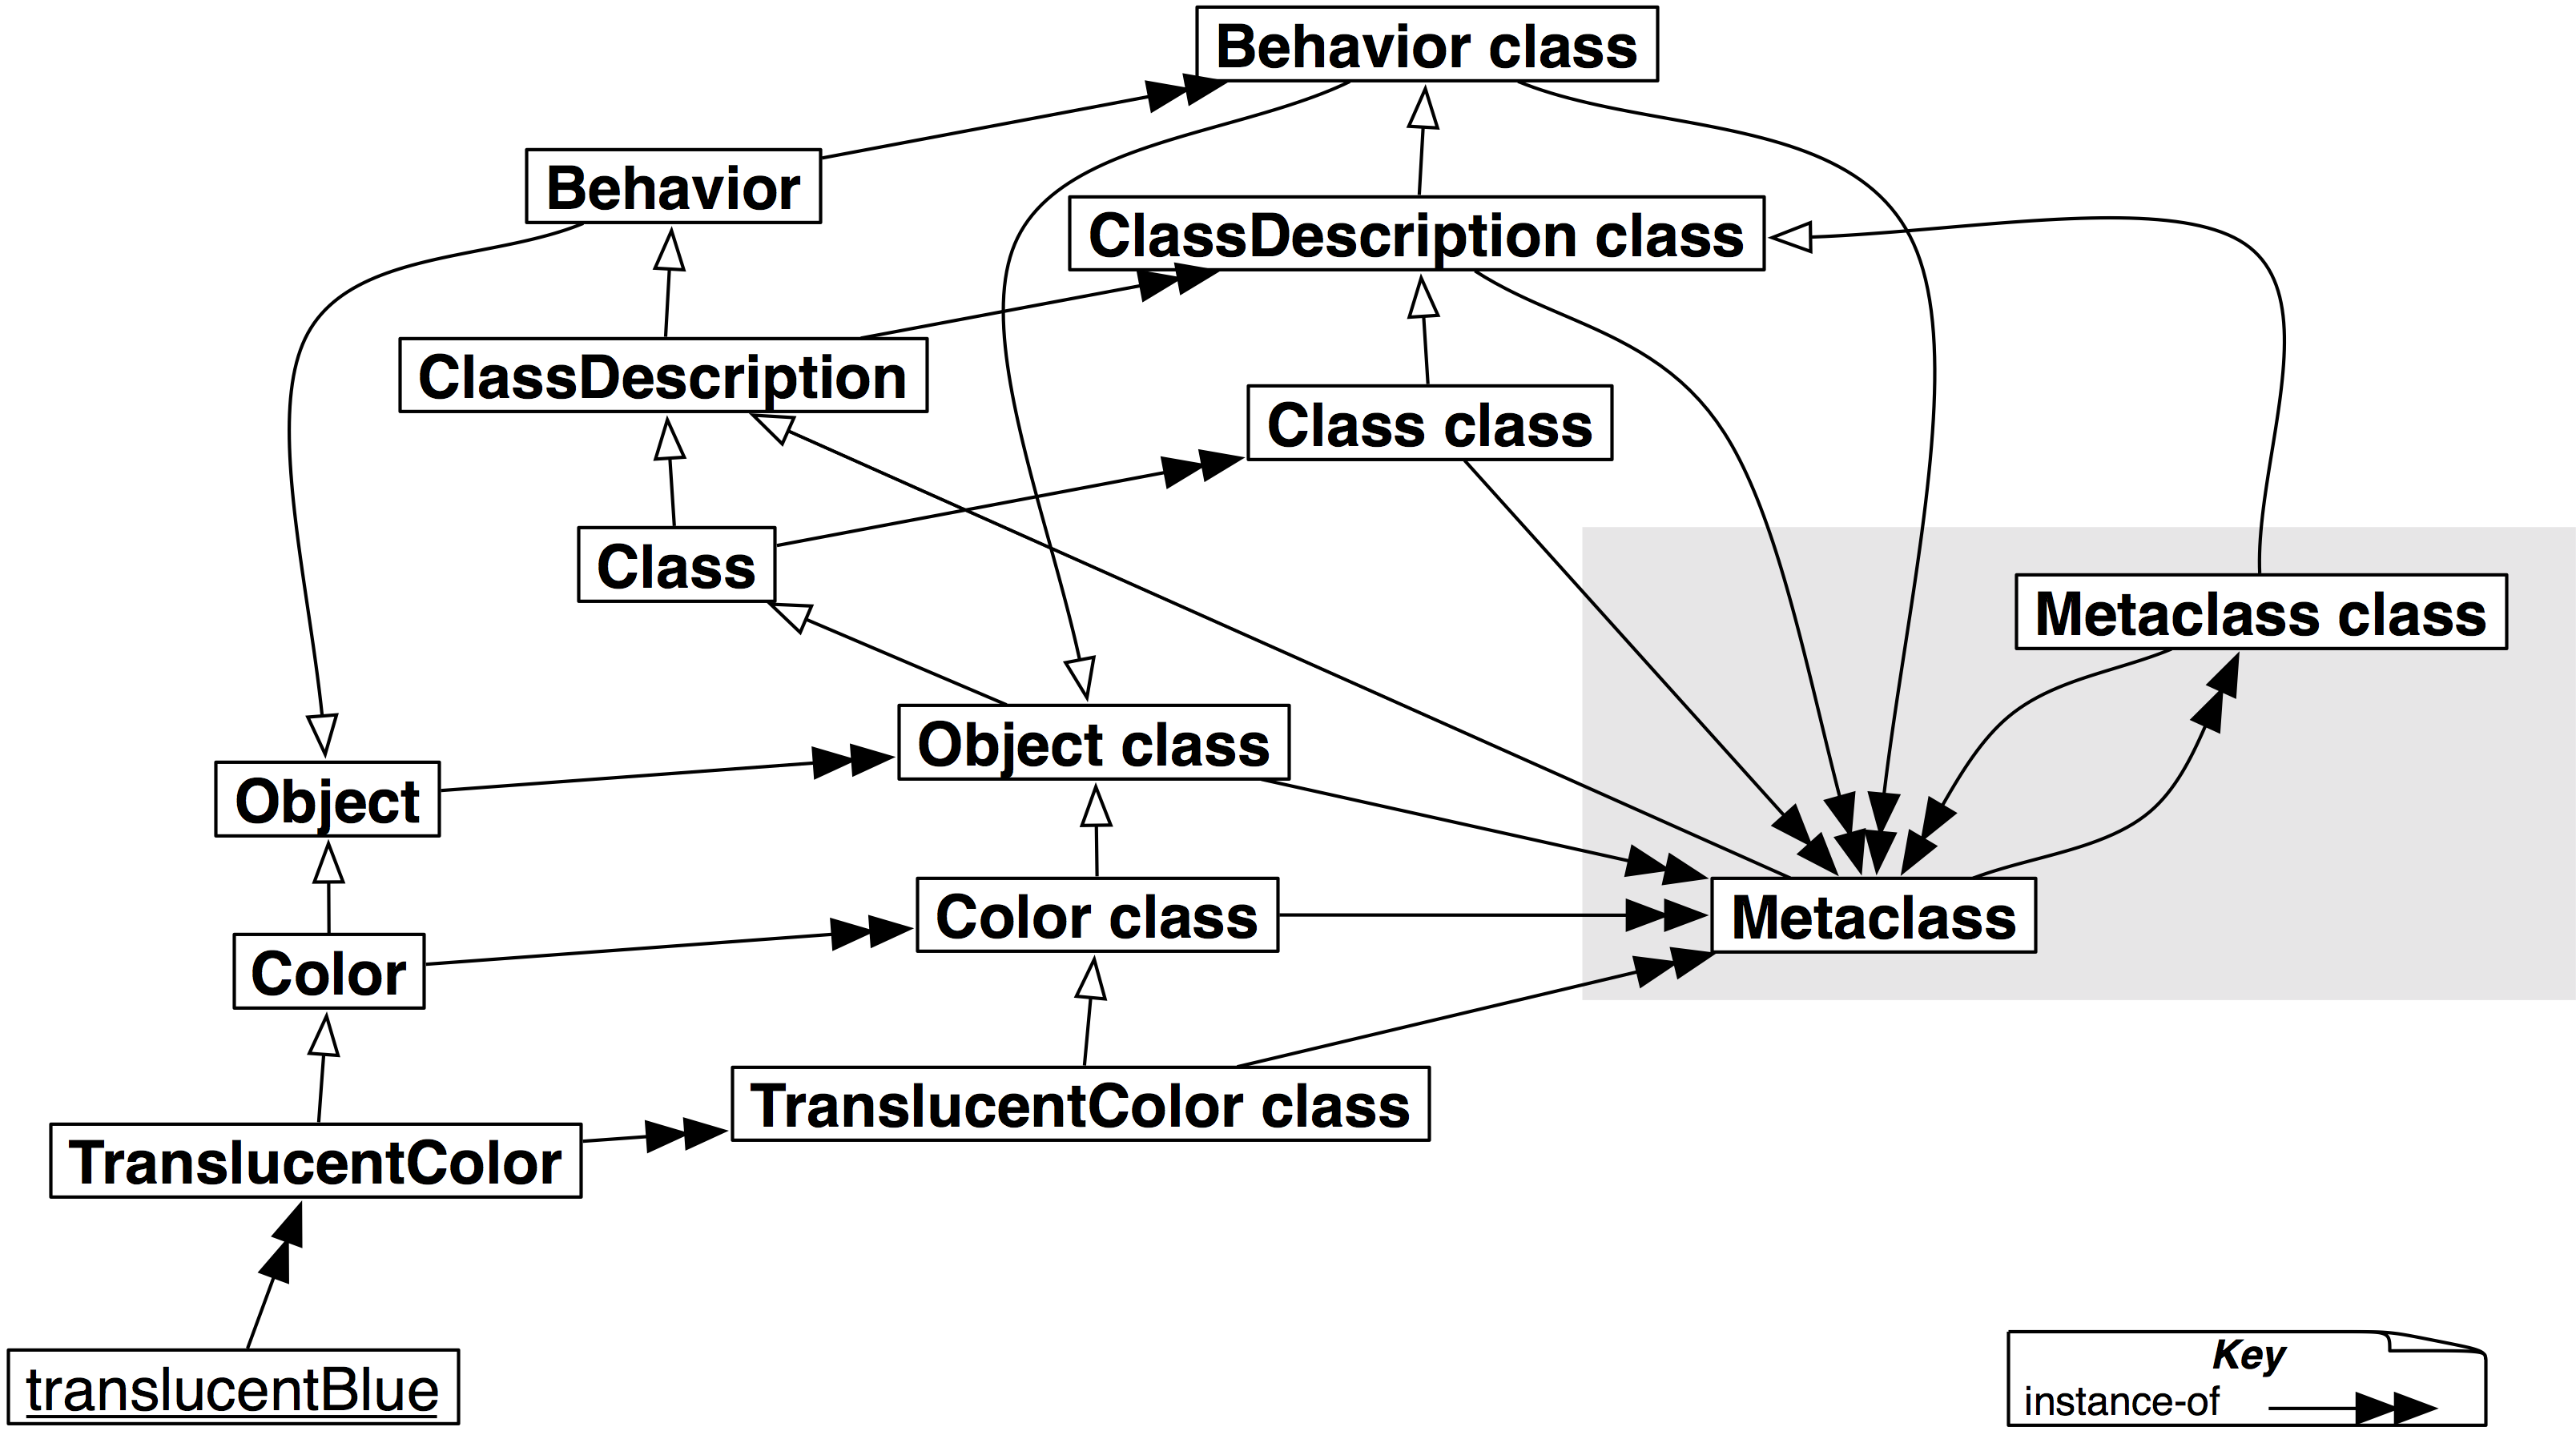
\includegraphics[width=120mm]{./img/smalltalk_class_hierarchy.png}
\vspace{20pt}

Quite complex and in some areas even a little confusing. Smalltalk's approach that everything is an instance of some class poses a question where does it end? Most languages that introduce a concept of a metaclass have to solve this by a loop: in Smalltalk's case, it is the loop between \verb=Metaclass= and \verb=Metaclass class=, where each is an instance of the other. The Objective-C object model indeed has a similar loop, however, isn't that complex and generally ends at the \verb=Object class= point in the Smalltalk diagram.

\paragraph{Root Class}
\verb=NSObject= class is part of the Foundation framework Apple supplies. While it is often assumed to be the one and only root class in Objective-C, this is quite incorrect: there can be as many root classes in Objective-C as you wish - \verb=NSProxy= is an example and you can easily create your own:

\begin{verbatim}@interface ClassWithoutSuperclass {
  
}

@end\end{verbatim}

This will declare a new root class. It has absolutely no functionality - no memory management methods such as \verb=-retain= and \verb=-release=, no \verb=+alloc= method is declared either - you wouldn't be able to even create a new instance of this class without the run-time function \verb=class_createInstance= - which is basically why it is recommended to inherit all classes from NSObject (or any other already prepared root class) which implements some basic communication with the run-time as well as some basic memory management, etc. Also Apple's run-time has hardcoded references to \verb=NSObject=, which enables faster ARR message dispatch (as it checks if the class has any custom ARR-method implementation).

In Objective-C, each object is a pointer to a structure, where the first member is a so-called \verb=isa= pointer. Actually, the \verb=id= type, that represents any Objective-C object is defined as follows:

\begin{verbatim}
typedef struct objc_class *Class;
typedef struct {
  Class isa;
} *id;
\end{verbatim}

To support the behavior that a class (\ver=Class=) is an object as well, the class structure begins with the \verb=isa= pointer as well, which points to its meta class. The \verb=isa= pointer is followed by a \verb=superclass= field and many others - ivars, methods, cache, dispatch table, etc. - depending also on the run-time that you are using - you should hence never rely on the class structure itself, it should be treated as an opaque structure, with the internals exposed only to the run-time itself. To simplify this example, let's use this simplified class structure:

\begin{verbatim}
typedef struct class_t {
  struct class_t *isa;
  struct class_t *superclass;
  
  // Actually, more fields follow
} objc_class_t;
\end{verbatim}

For a regular class, the \verb=isa= pointer points to its meta class and the \verb=superclass= pointer points to its regular superclass, or \verb=Nil= in case it is the root class (in Objective-C, the zero pointer is called \verb=nil= for objects and \verb=Nil= for classes - both are just a \verb=#define=s of a typed zero, though). Now how about the meta class?
In case the class isn't a root class, the \verb=superclass= pointer points to its meta superclass and the \verb=isa= pointer points to the same meta superclass. Hence the regular class is an instance of its superclass. In case the class is a root class, its \verb=isa= pointer points to the structure itself, and its superclass is the regular class. Let's examine this on an example:

\begin{verbatim}@interface Rootclass{
  
}

@end

@implementation Rootclass

// Empty implementation

@end



@interface Subclass : Rootclass{

}

@end

@implementation Subclass

// Empty implementation

@end 
\end{verbatim}

This declares two classes (actually four, as for each class a meta class is created as well) - \verb=Rootclass= and \verb=Subclass=. The \verb=Rootclass= is a new root class with no superclass. As neither of these classes declares any methods, calling anything on either class would result in a run-time exception, even the usual object creation via \verb=[[Rootclass alloc] init]= isn't available as \verb=Rootclass= doesn't declare the \verb=+alloc= method - it's declared on the \verb=NSObject= class, which is why you can create instances of the ``regular" classes inheriting from \verb=NSObject= this way.

Hence we need to use the run-time \verb=class_createInstance= function to create an instance of the class:

\begin{verbatim}
id obj = class_createInstance(objc_getClass("Subclass"), 0);
\end{verbatim}

The \verb=objc_getClass= function returns a pointer to the class called \verb=Subclass=, the \verb=class_createInstance= function creates an instance of the \verb=Subclass= class, with \verb=0= extra bytes - the extra bytes parameter is here in case you wanted to dynamically add extra space to some of your instances, or to all by overriding the \verb=+alloc= method of the class (it is noteworthy that the \verb=+alloc= method is actually nothing else than \verb=-alloc= on the meta class - i.e.\ all class methods are in fact instance methods on the meta class).


When we try to visualize this situation (two classes - one root class and its subclass; and an instance of the subclass), we get a diagram that can be seen on figure \~ref{fig:class_metaclass_graph}.


\begin{figure}[htbp] 
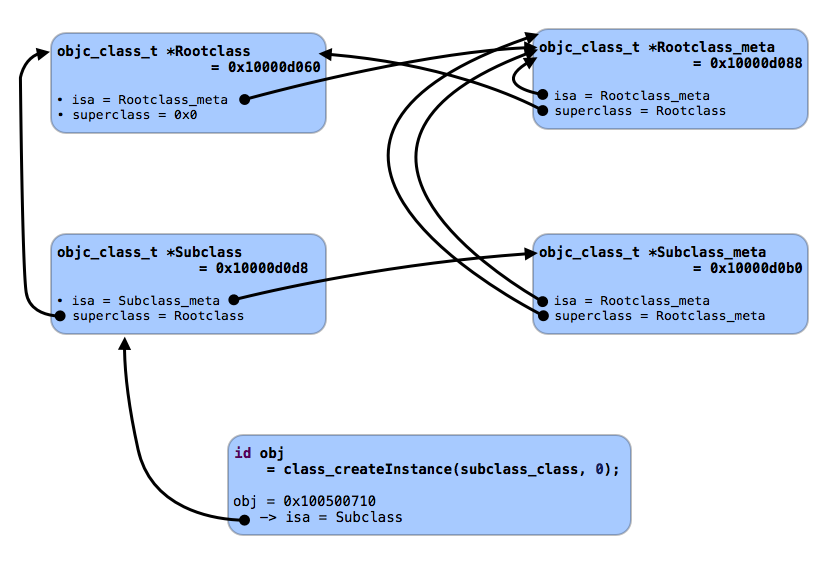
\includegraphics[width=\textwidth]{img/metaclass_graph.png}
  \centering{}
  \caption{A graph of the class - meta-class relationship.}
  \label{fig:class_metaclass_graph}
\end{figure}

As you can see, it is far less complicated than the Smalltalk object model. The class hierarchy ends at the point of the root class. To sum it up:

\begin{itemize}
\item Each class consists actually of two classes: the regular class and the meta class.
\item As the class hierarchy goes, the meta class hierarchy follows the regular class hierarchy up to the root class.
\item The root class is a little special, as the meta class is an instance of itself and its superclass is the regular class (which is an instance of the meta class).
\item It is easy to detect a meta class - \verb:cl == cl->isa:.
\item This has a peculiar consequence: all instance methods of the root class are class methods as well (in the lookup chain, when the search on meta classes yields nothing, the run-time follows the \verb=superclass= pointer, which points to the regular class object). This can be easily verified:
\end{itemize}

\begin{verbatim}
unsigned int number_of_methods = 0;
Method *methods, *method_ptr;
methods = method_ptr = class_copyMethodList([NSObject class], 
                                            &number_of_methods);
while (number_of_methods){
  printf("%s\n", sel_getName(method_getName(*methods)));
  ++methods;
  --number_of_methods;
}
free(method_ptr);
\end{verbatim}

This piece of code prints all available methods on a class. The \verb=[NSObject object]=, however, is the regular class, which on my installation of OS X prints out 298 methods (note that these are methods directly implemented by that class). If we replace \verb=[NSObject class]= with

\begin{verbatim}
methods = method_ptr = class_copyMethodList(
                                ((id)[NSObject class])->isa, 
                                &number_of_methods
                                           );
\end{verbatim}

we get a list of methods declared directly on the meta class. This list counts only 118 methods, among which, for example, isn't a method \verb=isNSArray__=, which is a private \verb=NSObject= instance method for deciding whether the object is of \verb=NSArray= class. While the meta class itself doesn't implement this, however, calling

\begin{verbatim}
[((id)[NSObject class])->isa isNSArray__];
\end{verbatim}

doesn't yield in any run-time exception, or similar, it simply invokes the instance method. This can be further proved by exchanging the function pointer of \verb=NSObject='s \verb=isNSArray__= method with your own function, that prints a message, for example.

While this trickery might be viewed as unnecessary and almost 'insane', it has a good reasoning behind - it is mostly because of this that you can treat classes as regular objects.

\subsection{Creating Classes Programmatically}

While this isn't a feature of the run-time you'd use on a daily basis, classes can be created and inserted into the run-time at any time. There is a function called \verb=objc_allocateClassPair= which creates a brand new class and its meta class counterpart - together a class pair. All you need to specify is the superclass, new class name and extra bytes (these extra bytes are similar to the extra bytes argument of \verb=objc_createInstance=, but now you are defining extra bytes on the class structure itself for possible class functionality extension). Run-time functions such as \verb=class_addMethod=, \verb=class_addIvar=, \verb=class_addProtocol= and \verb=class_addProperty= can be used to add methods, ivars, protocols and properties to a class.

Creating the class using \verb=objc_allocateClassPair= function isn't enough in order to create an instance of this class, though, as you need to register the class pair with the run-time as well using \verb=objc_registerClassPair=. This is simply to avoid creating an instance of the class before it gets fully initialized, e.g.\ from a different thread. Using these methods, you can easily substitute the Objective-C compiler, creating all classes at the beginning of the program execution.

In reality, declaring a class doesn't cause the compiler to generate function calls, however, instead, the compiler creates static class structures which are later on copied by the linker into the \verb=__OBJC= section of the Mach-O binary (on OS X), which is copied on the launch time to memory and the classes just get registered by the run-time (the dynamic loader calls some private run-time methods for copying classes from binary images), which is much faster that dynamically create classes one by one, connecting all methods, ivars, etc. We will, however, focus on the run-time methods, ignoring linker dependencies.

\subsection{Translating Methods to Functions}

As noted several times before, all Objective-C code can be rewritten in pure C code. This brings us to a question, how are the methods translated to C constructs - obviously into a function, so-called \verb=IMP= (an implementation pointer). Let's use this class to demonstrate:

\begin{verbatim}

@implementation SomeClass
+(void)doSomethingStatic{
  // ...
}
-(void)someMethod:(void*)arg1 secondArgument:(void*)arg2{
  // ...
}
@end

\end{verbatim}

This gets translated into two functions:

\begin{verbatim}
typedef struct objc_object SomeClass;

void _C_SomeClass_doSomethingStatic(Class self, SEL _cmd){
  // ...
}

void _I_SomeClass_someMethod_secondArgument(SomeClass *self,
                             SEL _cmd, void *arg1, void *arg2){
  //...
}
\end{verbatim}

As you can see, each method gets translated into a function of at least two arguments. The first argument is \verb=self= - a pointer to the object the message is being sent to. In the first case a \verb=Class= object, in the second case a pointer to the \verb=SomeClass= object. The second argument, \verb=_cmd=, is the selector (\verb=SEL=). If you have a function with this signature, you can easily exchange method implementations of existing methods, or add methods of your own.

The function names get slightly obfuscated - \verb=_X_ClassName_method_name_= - where \verb=X= is either \verb=I= for instance methods or \verb=C= for class methods. As Objective-C method names can have multiple parts, each followed by a semi-colon (e.g.\ \verb=someMethod:secondArgument:=), each part gets concatenated using an underscore.

\subsection{Synchronization}

Objective-C has a \verb=@synchronize(obj)= syntax, which locks a recursive mutex associated with \verb=obj= at the beginning of the synchronization scope and unlocks it at the end. For example:

\begin{verbatim}
...

@synchronized(self){
  // Critical code goes here
}
...
\end{verbatim}

gets rewritten into:

\begin{verbatim}
...
objc_sync_enter((id)self);
@try{
  // Critical code goes here
}
@finally (id exception){
  objc_sync_exit((id)self);
}
...
\end{verbatim}

As you can see, to avoid deadlocks in case of exceptions, the synchronization \verb=objc_sync_enter= and \verb=objc_sync_exit= needs to be wrapped in \verb=@try-@finally= (no catching must be performed as the exception might need to be caught in a call above in the stack trace). Note that each object doesn't have its own lock (in the \'Etoil'e run-time it does, though), but a pool of locks is used instead.

The \verb=@try-@catch-@finally= is, of course, again translated into C code, to be precise, the compiler uses the \verb=_setjmp= function to install a stack exception data and the run-time uses \verb=longjmp= function to throw exceptions - this is, however, only used for the old run-time - Apple's new run-time uses the C++ unwind library.

\subsection{Protocols}

Protocols are a way of declaring methods with no implementation that classes conforming to that particular protocol should implement. This mechanism is called \verb=interface= is Java, for example.

When a class conforms to a protocol, a pointer to a protocol is installed in its protocol list, which is quite obvious, but brings up a question, what is a protocol, in terms of structures.

Protocols are really nothing, but instances of internal class \verb=Protocol=:

\begin{verbatim}
@protocol SomeProtocol
-(id)protocolMethod;
@end


...
Class cl = objc_getClass("Protocol");
BOOL isProtocol = [@protocol(SomeProtocol) isKindOfClass:cl];
...
\end{verbatim}

The \verb=isProtocol= variable is set to \verb=YES=. Or, if you prefer this way:

\begin{verbatim}
printf(@"%s\n", class_getName(((id)@protocol(SomeProtocol))->isa));
\end{verbatim}

This prints out, indeed, \verb=Protocol=. Interestingly enough, the

\begin{verbatim}@protocol(SomeProtocol)\end{verbatim}
  
construct isn't simply translated to

\begin{verbatim}objc_getProtocol("SomeProtocol")\end{verbatim}

but is translated into 

\begin{verbatim}(Protocol *)&_OBJC_PROTOCOL_SomeProtocol\end{verbatim}

- a pointer to a certain exported protocol structure, that is part of the binary (and this isn't an optimization because the protocol is declared in the same source file).

Of course, the run-time needs to populate the \verb=isa= pointers of each protocol when loading the binary.

\subsection{Required Classes}

There are several language constructs that are compiled directly into objects, requiring the run-time to include classes for these objects.

\paragraph{Strings} The regular \verb=char*= C strings in quotes are simply a pointer to a chunk of memory that is typed as an array of \verb=char=s, which by definition cannot be an object, as the first field of \verb=id= is an \verb=isa= pointer. Hence it cannot be treated as an object and has to be wrapped in an object representing an Objective-C string - hence the \verb=@"Objective-C String"= notation.

This poses a question what is the string compiled to.

\begin{verbatim}
NSString *myString = @"My String";
\end{verbatim}

This gets compiled into:

\begin{verbatim}
NSString *myString = (NSString *)&__NSConstantStringImpl_test_m_0;
\end{verbatim}

Now, what is \verb=__NSConstantStringImpl_test_m_0=? That is actually a static object:

\begin{verbatim}
static __NSConstantStringImpl 
        __NSConstantStringImpl_test_m_0 
        __attribute__ ((section ("__DATA, __cfstring"))) = 
         {
           __CFConstantStringClassReference,
           0x000007c8,
           "My String",
           9
         };
\end{verbatim}

So, we have something resembling an object - the first field is \newline{}\verb=__CFConstantStringClassReference=, which seems like something that could be the \verb=isa= pointer, following by a hexadecimal number (flags), the actual \verb=char*= string and length of this string. And indeed:

\begin{verbatim}
struct __NSConstantStringImpl {
  int *isa;
  int flags;
  char *str;
  long length;
};
\end{verbatim}

Apple's implementation takes advantage of the CoreFoundation framework and toll-free bridging (see Chapter 2), not including the constant string implementation in the run-time itself at all (thus forcing all Objective-C programs to link against the CoreFoundation and Foundation frameworks). The GCC implementation, on the other hand, includes a \verb=NXConstantString= class (unlike Apple's implementation, the run-time then needs to fill in the \verb=isa= pointers with actual class pointers at the run-time).

\paragraph{Blocks}

Apple has introduced lambda functions C language extension in OS X 10.6 - so called blocks:

\begin{verbatim}
void(^myBlock)(void *) = ^(void *arg){
  // Do something with the argument
};
\end{verbatim}

This declares an anonymous function that can be used even out of the current scope and the function itself can freely use variables from within the scope of the method where the block is declared in a read-only manner. For read-write access to variables, the variables need to be declared as \verb=__block=, which generally makes them static variables, allowing the block to modify the variable even when the program execution is already out of scope.

This simple block gets translated into this piece of code (some minor changes to the code have been made to improve readability):

\begin{verbatim}
struct __block_impl {
  void *isa;
  int Flags;
  int Reserved;
  void *FuncPtr;
};


struct __myBlockImpl {
  struct __block_impl impl;
  struct __myBlockDescription *Desc;
  __myBlockImpl(void *fp, struct __myBlockDescription *desc, 
                                                int flags=0) {
    impl.isa = &_NSConcreteStackBlock;
    impl.Flags = flags;
    impl.FuncPtr = fp;
    Desc = desc;
  }
};

static void __myBlock_block_fnc(struct __myBlockImpl *__cself, 
                                                    void *arg){
  // Do something with the argument
}

static struct __myBlockDescription {
  unsigned long reserved;
  unsigned long Block_size;
} __myBlockDescription_DATA = { 0, sizeof(struct __myBlockImpl) };

...

void(*myBlock)(void *) = &__myBlockImpl(__myBlock_block_fnc, 
                                      &__myBlockDescription_DATA);

\end{verbatim}

While this indeed seems like a lot of fuzz for a block that does nothing, the actual mechanism behind is a lot more intriguing once you start using variables from within the scope inside the block - then all the variables get copied over into \verb=__myBlockImpl= (that's why the \verb=Block_size= gets assigned \verb=sizeof(=\verb=struct= \verb=__myBlockImpl)= as the \verb=_myBlockImpl= can be as large as possible depending on the number of variables used within the block).

Apart from the C++ usage (the structure constructor), the noteworthy part is the \verb=impl= field of \verb=__myBlockImpl= - which begins with an \verb=isa= pointer which is (again) filled with a specific class pointer. This allows the structure to be sent ARR methods, and hence be treated as an object, allowing it to be added to the \verb=NSArray= and \verb=NSDictionary= collections.
